\documentclass[Main]{subfiles}
\begin{document}

\subsection{Klassediagram}
Baseret på foregående Use Case-analyser kan det statiske klassediagram på Figur \ref{Fig:UML} udledes.
Systemet har flere, men de viste er de vigtigste der bruges af systemet og som der er udviklet mest på.


\begin{figure}[H]
\centering
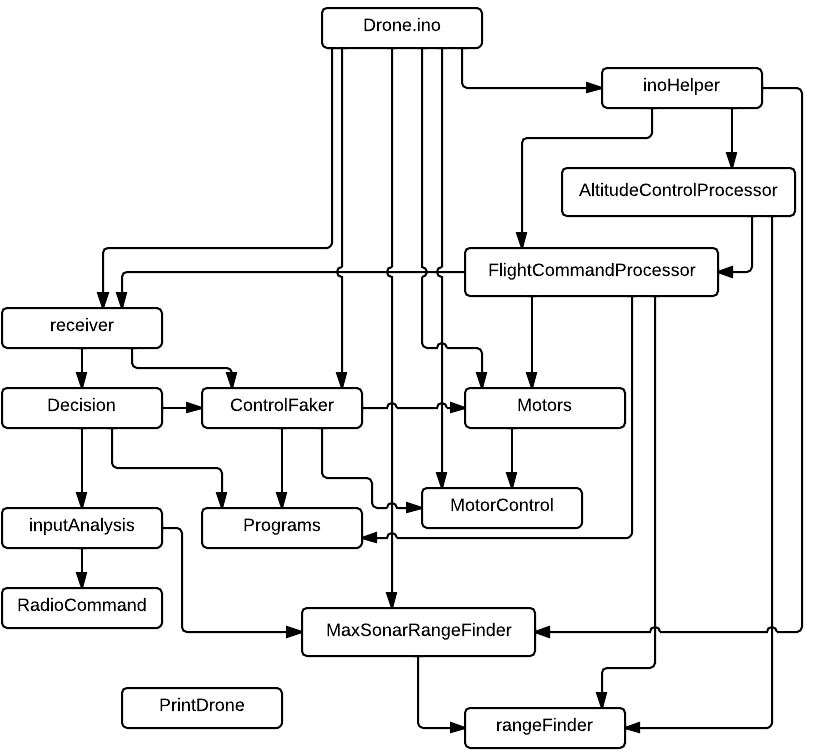
\includegraphics[scale=0.6]{UML}
\caption{Udsnit af det samlede klassediagram}
\label{Fig:UML}
\end{figure}

\newpage
\subsection{Klassebeskrivelser}
\subsubsection{Drone.ino}
\code{Drone.ino} er hovedfilen for systemet og har ikke fået foretaget de store ændringer i forhold til den oprindelige kode.
Denne fil skal indeholde de to obligatoriske funktioner \code{void setup()} og \code {void loop()}, da dette er hvad Arduino kører som den første og anden funktion.
Funktionen \code{void loop()} er i grove træk tilsvarende til et \code{while(1)}-loop, der ikke kan stoppes.
\\
Først nulstilles de fleste af klasserne herfra, hvorefter et schedulerings-system startes med en timer, der ser på 100Hz-, 50Hz-, 3 forskellige 10Hz-, 2Hz og 1Hz-funktioner skal køres. 
Disse er vigtige for systemets opbygning, da dette tillader udskrift via serial-forbindelsen til debugging og fordi den kun har én tråd til håndtering af funktioner.

\begin{Function}
\name{initPlatform}
\para{void}
\retu{void}
\comm{Denne funktion mapper LED'er som in-/output og starter \itoc forbindelsen.}
\end{Function}


\begin{Function}
\name{measureCriticalSensors}
\para{void}
\retu{void}
\comm{Denne funktion gør kald til de vigtigste sensorer (gyrometer og accelero\-meter)}
\end{Function}


\begin{Function}
\name{Setup}
\para{void}
\retu{void}
\comm{Arduino's første obligatoriske funktion -- Starter og reset'er de fleste filer og klasser: \\
Baudrate for serial port, læsning fra EEPROM, kald til \code{initPlatform()}, initierer motorer, ControlFaker, Receiver, Gyro (samt kalibrering), accelerometer, PID-værdier, kinematics, barometeret, sonarsensorerne samt nogle initieringsværdier for funktionen \code{loop()} og receiver'en. }
\end{Function}



\begin{Function}
\name{loop}
\para{void}
\retu{void}
\comm{Arduino's anden obligatoriske funktion: Denne svarer til en main-funktion med et \code{while(1){}} loop. 
\\ 
For hvert loop måles den nuværende tid som timestamp og sammenlignes med den sidste, så den ved hvor lang tid der er gået.
Så kaldes \code{measureCriticalSensors()}, da disse er kritiske for dronens stabilitet.
\\
Herefter inkrementeres \textit{FrameCounter}, der afgør hvornår fremtidige funktioner skal køres.
\textit{FrameCounter} indikerer, om der skal køres en 100-, 50-, tre forskellige 10-, 5-, eller 1-Hz funktion.
I slutningen af loopet sættes det sidste timestamp som den forrige tid, og hvis der er brug for det nulstilles \textit{FrameCounter}.}
\end{Function}


\class{inoHelper}
\code{inoHelper}-klassen er en hjælpefil der blev lavet til \code{drone.ino} på grund af dens uoverskuelige struktur og er den reelle implementering for 100Hz-, 50Hz-, tre forskellige 10Hz-, 5Hz-, og 1Hz-funktionerne.
Ud over den oprindelige implementering fra \code{drone.ino} er her også implementeret en masse debug-funktioner, som bruges til at måle alt fra sonarer input og motorer output til de falske værdier der sender til receiveren for at styre dronen efter ønske.


\begin{Function}
\name{initializePlatformSpecificAccelCalibration}
\para{void}
\retu{void}
\comm{Denne funktion indeholder nogle dummy-værdier for accelerometret, men disse overskrives af \code{EEPROM}-klassens gemte værdier fra den reelle kalibrering.}
\end{Function}


\begin{Function}
\name{process100HzTask}
\para{void}
\retu{void}
\comm{Denne funktion beregner flere af de vigtige værdier for dronens stabilitet, herunder kald til gyroskopet, accelerometret, barometret og beregning af dronens hastighed.
\\
Derudover kaldes \code{FlightControlprocessor}-klassens funktion \code{ProcessFlightControl()}.}
\end{Function}


\begin{Function}
\name{process50HzTask}
\para{void}
\retu{void}
\comm{Denne funktion starter læsningen af kommandoer der skal udføres og opdaterer sonarsensorerne.}
\end{Function}


\begin{Function}
\name{process10HzTask1}
\para{void}
\retu{void}
\comm{Denne funktion er blevet overflødig, da den kun gør noget med en kompassensor på.}
\end{Function}


\begin{Function}
\name{process10HzTask2}
\para{void}
\retu{void}
\comm{Denne funktion læser serialporten for kommandoer, der bruges til debugging, samt sender svar retur fra dronen.}
\end{Function}


\begin{Function}
\name{process10HzTask3}
\para{void}
\retu{void}
\comm{Denne funktion laver en timestamp-opdatering for kinematic-funktionerne.}
\end{Function}


\begin{Function}
\name{process2HzTask}
\para{void}
\retu{void}
\comm{Denne funktion udskriver forskellige debug-information 2 gange i sekundet, herunder sonarsensorernes målinger, om disse er advarsler, det valgte program og styringsinput.}
\end{Function}


\begin{Function}
\name{process1HzTask}
\para{void}
\retu{void}
\comm{Denne funktion udskriver forskellige debug-information 1 gange i sekundet.}
\end{Function}


\begin{Function}
\name{PrintChosenProgram}
\para{void}
\retu{static void}
\comm{Denn funktion udskriver det valgte program.}
\end{Function}


\begin{Function}
\name{PrintSonarReport}
\para{void}
\retu{static void}
\comm{Denne funktion udskriver gennemsnitsværdien for de sidste målinger af sonarsensorerne og om dronen flyver i fri højde eller i en fixeret højde.}
\end{Function}


\begin{Function}
\name{PrintAltitudeReport}
\para{void}
\retu{static void}
\comm{Denne funktion udskriver, om dronen kan se sonarsensoren på maven og om den er i panic-mode.}
\end{Function}


\begin{Function}
\name{PrintDebugReport}
\para{void}
\retu{static void}
\comm{Denne funktion udskriver om motorerne er aktiveret.}
\end{Function}


\begin{Function}
\name{PrintWarnings}
\para{void }
\retu{static void}
\comm{Denne funktion udskriver sonarsensorernes advarsler, såfremt der er nogle.}
\end{Function}


\begin{Function}
\name{PrintControllerOutput}
\para{void}
\retu{static void}
\comm{Denne funktion udskriver receiver-input i form af x-, y- og z-aksen, gaspedalen og om den skal holde en bestemt højde.}
\end{Function}


\class{FlightCommandProcessor}
\code{FlightCommandProcessor}-klassen er skrevet af AeroQuad og holder styr på de signaler der kommer fra \code{Receiver}-klassen og bruger disse input til at justere hardwaren ved opstart og beregne hvor meget langt der skal være til jorden for autoland- og hover-kommandoerne.


\begin{Function}
\name{isPositionHoldEnabledByUser}
\para{void}
\retu{bool}
\comm{Checker, om hover-funktionen er aktiveret. 
Hvis den er, returnere \code{true} -- ellers \code{false}}
\end{Function}


\begin{Function}
\name{processAltitudeHoldStateFromReceiverCommand}
\para{void}
\retu{void}
\comm{Såfremt hover-funktionen er aktiveret og dronen ikke flyver vildt, vil højden dronen skal holde blive læst ind i PID'en til senere beregninger.}
\end{Function}


\begin{Function}
\name{processAutoLandingStateFromReceiverCommand}
\para{void}
\retu{void}
\comm{Såfremt autoland-funktionen er aktiveret og dronen ikke flyver vildt, vil barometret og gyroskopets værdier blive læst ind i PID'en til senere beregninger.}
\end{Function}


\begin{Function}
\name{processZeroThrottleFunctionFromReceiverCommand}
\para{void}
\retu{void}
\comm{Kaldes, når gaspinden er i bund.
Dette kan derefter aktivere motorerne, kalibrere gyroskopet, accelerometeret og læse værdier fra \code{EEPROM}-klassen, samt udføre et sikkerhedscheck.}
\end{Function}


\begin{Function}
\name{readPilotCommands}
\para{void}
\retu{void}
\comm{Starter læsning af nyt værdier til \code{Receiver}-klassen og kalder de andre funktioner i \code{FlightCommandProcessor}-klassen}
\end{Function}




\class{Receiver \label{sec:receiver}}
\code{Receiver}-klassen styrer hvilke værdier der skal sendes til motorerne ved at læse input fra \code{ControlFaker-klassen} (afsnit \ref{sec:controlFaker}) og lader \code{Decision}-klassen (afsnit \ref{sec:decision}) træffe beslutning herom.


\begin{Function}
\name{initializeReceiverValues}
\para{void}
\retu{void}
\comm{Nulstiller alle værdier.}
\end{Function}


\begin{Function}
\name{initializeReceiverParam}
\para{int = 6 (default værdi)}
\retu{void}
\comm{Nulstiller alle værdier der skal skrives til motoren og de hjælpevariabler der bruges.}
\end{Function}


\begin{Function}
\name{readReceiver}
\para{void}
\retu{void}
\comm{Udfører inden flyvning en masse sikkerhedscheck og nulstillinger af andre filers variabler.
Efter dette checkes om dronen flyver for højt, hvilket program der bør køres, aktiverer programmet og slukker for dronen hvis nødvendigt pga. data in- og output.}
\end{Function}


\begin{Function}
\name{ApplyData}
\para{void}
\retu{void}
\comm{Behandler værdierne der skal sendes til motorerne.}
\end{Function}


\begin{Function}
\name{getReceiverSIData}
\para{byte}
\retu{const float}
\comm{Skallering af data for motorerne.}
\end{Function}


\begin{Function}
\name{PrintReceiverOutput}
\para{void}
\retu{void}
\comm{Udskriver værdier der sendes videre til motorerne}
\end{Function}



\class{Decision \label{sec:decision}}
\code{Decision}-klassen er lavet til at afgøre, hvilket program der skal køres, på baggrund af \code{InputAnalysis}-klassen (afsnit \ref{sec:inputAnalysis}).


\begin{Function}
\name{ResetMessages}
\para{void}
\retu{void}
\comm{Nulstiller alle variabler i filen.}
\end{Function}


\begin{Function}
\name{GetActualProgram}
\para{void}
\retu{ProgramInput}
\comm{Returnerer det aktuelle program}
\end{Function}


\begin{Function}
\name{SerialComRequest}
\para{ProgramInput}
\retu{void}
\comm{Læser hvilket program der skal køres fra serial-porten.}
\end{Function}


\begin{Function}
\name{ResetDecisions}
\para{void}
\retu{void}
\comm{Kalder nulstilling af \code{InputAnalysis}-klassen (afsnit \ref{sec:inputAnalysis}).}
\end{Function}


\begin{Function}
\name{PrintWarnings}
\para{void}
\retu{static void}
\comm{Udskriver hvilken sonar der er advarsel på, såfremt der er en.}
\end{Function}


\begin{Function}
\name{SonarCheck}
\para{void}
\retu{static void}
\comm{Afgør hvad der skal ske med advarslerne fra sonarsensorerne og hvilke programmer der skal køres.}
\end{Function}


\begin{Function}
\name{ProcessSignal}
\para{void}
\retu{static void}
\comm{Sikre valg af autoland- og start-program fra serial-porten og radioen. 
Såfremt disse ikke vælges læses det aktuelle program.}
\end{Function}


\begin{Function}
\name{DecideProgram}
\para{void}
\retu{void}
\comm{Kaldes fra \code{Receiver}-klassen (afsnit \ref{sec:receiver}) til at foretage analysen.
Funktionen kalder ned i \code{InputAnalysis}-klassen (afsnit \ref{sec:inputAnalysis}) for sonarsensorernes input.}
\end{Function}



\begin{Function}
\name{SelectProgram}
\para{int}
\retu{static void}
\comm{Aktiverer det ønskede program og lader de enkelte programmer mulige at kalde mens hover-funktionen er aktiveret.}
\end{Function}


\begin{Function}
\name{TimeSpend}
\para{Timers}
\retu{float}
\comm{Returnere en tid mellem dette kalds timestamp og det sidste i millisekunder.}
\end{Function}


\begin{Function}
\name{GroundTakeOff}
\para{void}
\retu{void}
\comm{Beregner en omvendt eksponentiel kurs for dronens throttle-værdi, som dronen kan lette med ved start-program.}
\end{Function}


\begin{Function}
\name{GroundStart}
\para{void}
\retu{void}
\comm{Inkrementerer langsomt dronens throttle-værdi, indtil den når den fastsatte værdi for det aktuelle program.}
\end{Function}


\begin{Function}
\name{IncreaseHeight}
\para{void}
\retu{void}
\comm{Inkrementerer den nuværende throttle-værdi med 10, hvis den ikke er blevet kaldt inden for de sidste 300 millisekunder.}
\end{Function}


\begin{Function}
\name{DecreaseHeight}
\para{void}
\retu{void}
\comm{Dekrementerer den nuværende throttle-værdi med 10, hvis den ikke er blevet kaldt inden for de sidste 300 millisekunder.}
\end{Function}


\begin{Function}
\name{HoldHeight}
\para{void}
\retu{void}
\comm{Læser den nuværende højde og sætter denne til det aktuelle programs højde, hvorefter hover-funktionen aktiveres og autoland-funktionen deaktiveres.}
\end{Function}


\begin{Function}
\name{MaxHeightAction}
\para{void}
\retu{void}
\comm{Læser den nuværende værdi og er den større end 100 cm aktiveres hover-funktionen og det aktuelle program sættes til 60 cm højde.}
\end{Function}



\class{InputAnalysis \label{sec:inputAnalysis}}
\code{InputAnalysis}-klassen står for at behandle de signaler der læses fra sonarsensorerne, samt input fra \code{RadioCommand}-klassen (afsnit \ref{sec:radioCommand}).

\begin{Function}
\name{ResetInputAnalysis}
\para{void}
\retu{void}
\comm{Nulstiller lokale variabler og kalder nulstilling af \code{RadioCommand}-klassen (afsnit \ref{sec:radioCommand}).}
\end{Function}


\begin{Function}
\name{AnalyseSonarInput}
\para{void}
\retu{void}
\comm{Dronen sætter advarselsflag for sonarsensorerne, hvis anstanden bliver for lille, der kan kan aflæses af \code{Decision}-klassen (afsnit \ref{sec:decision}).}
\end{Function}


\begin{Function}
\name{AnalyseRadioInput}
\para{void}
\retu{void}
\comm{Kalder analyse af radioprogram og sætter variable med dette.}
\end{Function}


\begin{Function}
\name{GetRadioProgram}
\para{void}
\retu{int}
\comm{Returnere det aktuelle radioprogram.}
\end{Function}


\begin{Function}
\name{GetLeftWarning}
\para{void}
\retu{bool}
\comm{Returnere advarsel fra venstre sonarsensorer.}
\end{Function}


\begin{Function}
\name{GetRightWarning}
\para{void}
\retu{bool}
\comm{Returnere advarsel fra højre sonarsensorer.}
\end{Function}


\begin{Function}
\name{GetFrontWarning}
\para{void}
\retu{bool}
\comm{Returnere advarsel fra front sonarsensorer.}
\end{Function}



\class{RadioCommand \label{sec:radioCommand}}
\code{Radiocommand}-klassen læser input fra radiomodtageren vha. \itoc og stiller resultatet til rådighed.
\begin{Function}
\name{SetupRadioCommunicaiton}
\para{void}
\retu{void}
\comm{Nulstiller lokale variabler og sætter kommunikationen til radioen op.}
\end{Function}


\begin{Function}
\name{ReadRadio}
\para{void}
\retu{void}
\comm{Aflæser radioens program og sætter sin globale værdi til denne.}
\end{Function}



\class{ControlFaker \label{sec:controlFaker}}
\code{ControlFaker} har ansvaret for inputtet til \code{Decision}-klassen (afsnit \ref{sec:decision}) og sørger samtidig for, at det input der sendes dertil af sikkerhedsmæssige årsager ikke overskrider fastsatte grænser.
\begin{Function}
\name{SetupControlFaker}
\para{void}
\retu{void}
\comm{Nulstiller lokale værdier og sørger for udskrivning gennem Serial-porten.}
\end{Function}


\begin{Function}
\name{KillMotor}
\para{void}
\retu{void}
\comm{Sender signal om at slukke for alle motorer, slukker alle output til Serial-porten og nulstiller dronens x-, y- og z-akse.}
\end{Function}


\begin{Function}
\name{ApplyProgram}
\para{void}
\retu{void}
\comm{Skriver \code{Programs}-klassen (afsnit \ref{sec:programs}) programværdier til de aktuelle værdier.}
\end{Function}


\begin{Function}
\name{ArmMotors}
\para{void}
\retu{void}
\comm{Sætter indstillinger for, at motorerne kan starte}
\end{Function}


\begin{Function}
\name{SafetyCheck}
\para{void}
\retu{void}
\comm{Sætter indstillinger for, at et sikkerhedscheck godkendes.}
\end{Function}


\begin{Function}
\name{PerformCalibration}
\para{void}
\retu{void}
\comm{Sætter indstillinger for, at dronen vil kalibrere sine sensorer.}
\end{Function}


\begin{Function}
\name{ApplySpeed}
\para{void}
\retu{void}
\comm{Hvis \code{KillMotor()} har været kaldt nulstilles x-, y- og z-aksen og throttle-værdien sættes til under minimumshastigheden for propelrotation. 
Hvis ikke checkes om nogle af motorerne roterer for hurtigt, hvilket resulterer i kald af \code{KillMotor()}.}
\end{Function}


\begin{Function}
\name{ResetFakerData}
\para{void}
\retu{void}
\comm{Nulstiller værdier der læses som aktuelle input af \code{Receiver}-klassen (afsnit \ref{sec:receiver}).}
\end{Function}


\class{Programs \label{sec:programs}}
\code{Programs}-klassen indeholder programmer til forskellige udførelser for dronen, heriblandt flyv frem, roter, op, ned, let, land mm.

\begin{Function}
\name{ResetProgramData}
\para{void}
\retu{void}
\comm{Nulstiller programværdierne for dronens program.}
\end{Function}


\begin{Function}
\name{ForwardSlow}
\para{void}
\retu{void}
\comm{Dronens program sættes til at flyve langsomt frem med fastdefineret fart i fastdefineret tid}
\end{Function}


\begin{Function}
\name{ForwardFast}
\para{void}
\retu{void}
\comm{Dronens program sættes til at flyve hurtigt frem med fastdefineret fart i fastdefineret tid}
\end{Function}


\begin{Function}
\name{RotateRightSlow}
\para{void}
\retu{void}
\comm{Dronens program sættes til at rotere til højre med fastdefineret fart i fastdefineret tid}
\end{Function}


\begin{Function}
\name{RotateLeftSlow}
\para{void}
\retu{void}
\comm{Dronens program sættes til at rotere til venstre med fastdefineret fart i fastdefineret tid.}
\end{Function}


\begin{Function}
\name{AutoLand}
\para{void}
\retu{void}
\comm{Aktiverer autoland-funktionen og overskriver rotation og fremdrift, så dronen forbliver stabil i luft.}
\end{Function}


\begin{Function}
\name{Start}
\para{void}
\retu{void}
\comm{Deaktiverer hover-funktionen så dronens throttle-værdien bestemmer højden.}
\end{Function}


\begin{Function}
\name{StopMidAir}
\para{void}
\retu{void}
\comm{Overskriver rotation og fremdrift, så dronen holder sig lige i luften.}
\end{Function}



\class{MotorControl \label{sec:motorControl}}
\code{MotorControl}-klassen er en simpel klasse, der kan kaldes fra alle andre klasser. 
Den har ingen afhængigheder til andre klasser og sætter et flag til at slukke for motorerne ved sat.

\begin{Function}
\name{KillMotor}
\para{bool}
\retu{void}
\comm{Sætter inputparameteren til hvorvidt motorerne skal være slukket eller ej.}
\end{Function}


\begin{Function}
\name{IsMotorKilled}
\para{void}
\retu{bool}
\comm{Returnerer motorernes nuværende status -- slukket eller ej.}
\end{Function}



\class{MaxSonarRangeFinder \label{sec:maxSonar}}
\code{MaxSonarRangeFinder}-klassen bestemmer hvilken sonar skal aflæses og gemmer gennemsnittet af de sidste par målinger for hver sonar.

\begin{Function}
\name{inititalizeRangeFinders}
\para{void}
\retu{void}
\comm{Nulstiller de lokale værdier samt sætter læsning af hardware pins til deres respektive værdier.}
\end{Function}


\begin{Function}
\name{updateRangeFinders}
\para{void}
\retu{void}
\comm{Læser én sonar og gemmer resultatet i en kø for den pågældende sonar.\\
Funktionen aflæser sonaren på maven af dronen hver anden gang; bunden -- venstre -- bunden -- front -- bunden -- højre\dots}
\end{Function}


\begin{Function}
\name{StoreRangeValues}
\para{int}
\retu{void}
\comm{Gemmer inputtets (sonarens) sidste måling i en FIFO-kø, skubber det sidste element ud og gemmer gennemsnittet af den nye kø.}
\end{Function}


\class{PrintDrone \label{sec:printDrone}}
\code{PrintDrone}-klassen udskriver beskeder til Serial-porten. 
Dette kan kan gøres ved at kalde en funktion der skriver på linjen, eller som skifter linje.
Foruden det kan der specificeres hvilket output man ønsker og alle meddelelser opdeles derfor i kategorier, som kan aktiveres og deaktiveres.

\begin{Function}
\name{SetupPrintDrone}
\para{void}
\retu{void}
\comm{Sætter alle kategorier til at kunne udskrive.}
\end{Function}

\begin{Function}
\name{SilenceSerial}
\para{void}
\retu{void}
\comm{Slukker for alle kategoriers output og husker hvilke der var aktive.}
\end{Function}

\begin{Function}
\name{ActivatePreviousSerial}
\para{void}
\retu{void}
\comm{Aktiverer de kategorier, der tidligere var tændte.}
\end{Function}

\begin{Function}
\name{printNewLine}
\para{int / float / double / unsigned long / String, printModes}
\retu{void}
\comm{Udskriver en besked eller et tal i den givende kategori og bliver på den nuværende linje.}
\end{Function}

\begin{Function}
\name{printInLine}
\para{int, long, String, char, float, unsigned long, printModes}
\retu{void}
\comm{Udskriver en besked eller et tal i den givende kategori og skifter derefter til en ny linje.}
\end{Function}

\code{Sender Radio}-klassen er den der står og lytter efter brugerinput. Når der så er et input, klargør den en pakke som skal sendes ved hjælp af 
radioen. Denne pakke sendes så til radioen som sender den videre ud som radiobølger.

\begin{Function}
\name{SPI MasterInit}
\para{void}
\retu{void}
\comm{Initialize SPI porten på ATmega8 som master, sætter clk raten til fck/16.}
\end{Function}

\begin{Function}
\name{CSn}
\para{int}
\retu{void}
\comm{Chip select for SPI porten.}
\end{Function}

\begin{Function}
\name{switchOn}
\para{unsigned char}
\retu{unsigned char}
\comm{Chekker om et givent ben er sat lav eller høj.}
\end{Function}


\begin{Function}
\name{SPI transmit}
\para{unsigned char}
\retu{unsigned char}
\comm{Starter transmissionen mellem µ-controlleren og radioen over SPI.}
\end{Function}

\begin{Function}
\name{SendProgram}
\para{void}
\retu{void}
\comm{Starter med at flushe radioen så der ikke kan ligge gamle data i output bufferen, sender så de nye data til den og starter transmissionen på radioen, venter til den har sendt alle data og sætter den i dvale igen. }
\end{Function}

\begin{Function}
\name{Full RegConfig}
\para{void}
\retu{void}
\comm{Sætter radioen op, eks. data hastighed, kanal valg, CRC check osv.}
\end{Function}

\begin{Function}
\name{main}
\para{void}
\retu{void}
\comm{Starter chippen op og køre alle opsætningerne, der er også en \code{while(1)}. 
Her bliver der hele tiden tjekket om nogle knapper bliver trykket på, hvis bliver der sendt en data pakke til radioen med en bestemt besked der skal sendes til modtageren.}
\end{Function}



\class{Modtager Radio\label{sec:Modtager}}

\code{Modtager Radio}-klassen er den der modtager et interrupt når der er kommet en pakke fra senderen, som den så henter fra radioen. Denne pakke bliver så lagt ud i en output buffer til dronen på \itoc porten.

\begin{Function}
\name{SPI MasterInit}
\para{void}
\retu{void}
\comm{Initialize SPI porten på ATmega8 som master, sætter CLK-raten til fck/16.}
\end{Function}

\begin{Function}
\name{CSn}
\para{int}
\retu{void}
\comm{Chip select for SPI porten.}
\end{Function}

\begin{Function}
\name{SPI transmit}
\para{unsigned char}
\retu{unsigned char}
\comm{Starter transmissionen mellem µ-controlleren og radioen over SPI.}
\end{Function}


\begin{Function}
\name{Full RegConfig}
\para{void}
\retu{void}
\comm{Sætter radioen op, eks. data hastighed, kanal valg, CRC-check osv.}
\end{Function}

\begin{Function}
\name{initExtInts}
\para{void}
\retu{void}
\comm{Enabler eksterne interrupts, så µ-controlleren kan få interrupts fra radioen.}
\end{Function}


\begin{Function}
\name{ISR INT0 vect}
\para{void}
\retu{void}
\comm{Interrupt rutinen der bliver kørt hver gang radioen har modtaget data, data bliver hentet og radioen sat til at lytte efter data igen.}
\end{Function}

\begin{Function}
\name{main}
\para{void}
\retu{void}
\comm{Starter chippen op og køre alle opsætningerne inc watchdog, der er også et \code{while(1)}-loop der servicere watchdogen og gør de nyeste data klar til \itoc interface.}
\end{Function}


\class{TWI slave\label{sec:TWI slave}}

\code{TWI slave}-klassen er den der modtager en forespørgsel fra dronen om data og sender svar retur. 

\begin{Function}
\name{TWI Slave Initialise}
\para{unsigned char}
\retu{void}
\comm{Sætter µ-controlleren op til \itoc slave.}
\end{Function}



\begin{Function}
\name{TWI Transceiver Busy}
\para{void}
\retu{unsigned char}
\comm{Tjekker om \itoc er linjen er optaget.}
\end{Function}

\begin{Function}
\name{TWI Get Data From Transceiver}
\para{unsigned char}
\retu{unsigned char}
\comm{Henter data fra \itoc buffer.}
\end{Function}


\begin{Function}
\name{TWI Start Transceiver With Data}
\para{unsigned char}
\retu{void}
\comm{Lægger et svar ud på \itoc porten.}
\end{Function}

\begin{Function}
\name{ISR TWI vect}
\para{void}
\retu{void}
\comm{Interrupt rutinen der bliver kørt når en start kommando bliver sendt på \itoc porten.}
\end{Function}


\end{document}
